\documentclass{article}
\usepackage[a4paper, total={6in, 9.5in}]{geometry}
\usepackage{enumitem}
\usepackage{amsthm}
\usepackage[makeroom]{cancel}
\usepackage{graphicx}
\graphicspath{ {./images/} }
\usepackage{amsfonts}

\begin{document}

\begin{center}
    \LARGE{Problem Set 7}\\[0.5em]
    \large{Levi Harrison}\\[0.5em]
    \small{December 4, 2023}
\end{center}

\,

\begin{enumerate}
    \item Prove Lemma 1: A countable UNION of finite sets is countable.
\end{enumerate}

\begin{proof}
    Take the finite sets, $A$, $B$, $C$, and so on. By definition, a finite set is countable as it contains a finite set of elements. So, if we take the union $A \cup B \cup C ...$, we can count all the elements by first numbering those in $A$: 1 through $|A|$, then those in $B$ but not in $A$: $|A|+ 1$ through $|A| + |B - A| + 1$, then those in $C$ but not in $B$ or $A$: $|A| + |B - A| + 2$ through $|A| + |B - A| + |C - (A \cup B)| + 2$ and so on. Thus, a union of finite sets is countable.
\end{proof}

\begin{enumerate}[resume]
    \item Prove Lemma 2: A countable UNION of countable sets is countable.
\end{enumerate}

\begin{proof}
    Take the countable sets $T_{1}$, $T_{2}$, $T_3$, ..., $T_n$ for $n \in \mathbb{N}$ (where all sets contain distinct elements from eachother). We can visualize the countable union (as $n \in \mathbb{N}$) of these sets, $\bigcup_{n = 1}^{\infty}T_n$, as follows, with each set having its own row, and each of element of each set represented as $T_{nm}$, where $n$ is the number of the set and $m$ being the number of the element in that set:

    \[T_1 = T_{1, 1}, T_{1, 2}, T_{1, 3}, ..., T_{1, m}\]
    \[T_2 = T_{2, 1}, T_{2, 2}, T_{2, 3}, ..., T_{2, m}\]
    \[T_3 = T_{3, 1}, T_{3, 2}, T_{3, 3}, ..., T_{3, m}\]
    \[...\]
    \[T_n = T_{n, 1}, T_{n, 2}, T_{n, 3}, ..., T_{n, m}\]

    To create an ordering scheme for the elements of this union, and thus prove the bijection between $\mathbb{N}$ and the union, we can number each element using alternating diagonals. So, the first element would be $T_{1, 1}$, the second $T_{1, 2}$, the third, $T_{2, 1}$, the forth $T_{3, 1}$, the fifth, $T_{2, 2}$, the sixth $T_{1, 3}$, and so on. Using diagonals, we can count every element in the union exactly once, and the existance of the bijection $\mathbb{N} \rightarrow \bigcup_{n = 1}^{\infty}T_n$ is proved. Thus, a countable union of countable sets is countable.
\end{proof}

\textit{Credit: Daniel}

\,

An infinite stairway is a path constructed by starting at the origin and then repeatedly drawing segments, either up one unit or to the right one unit. The stairway has height $h$ if it reaches $h$ units above the origin and remains there forever. (See the image below for an example of a stairway that looks like it has height 4; I say “looks” because the picture is truncated so maybe it rises again!)

\,

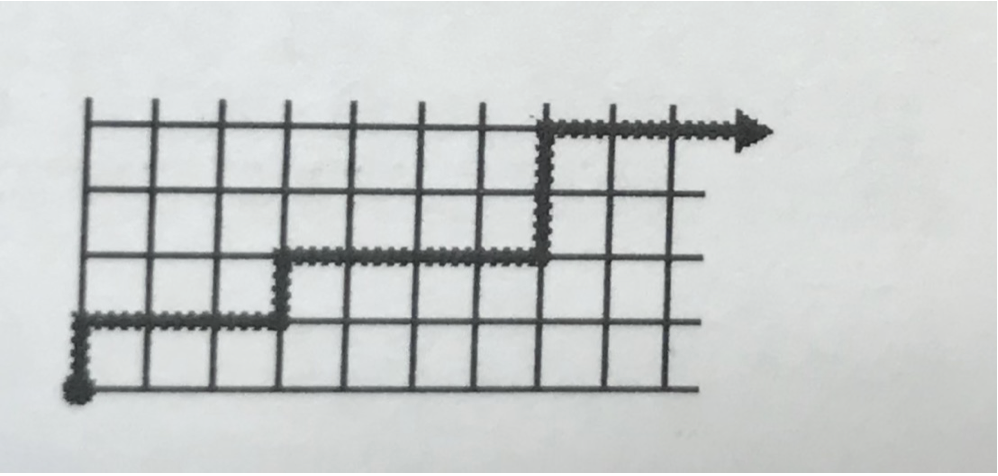
\includegraphics[scale=0.3]{problem 3}

\,

\begin{enumerate}[resume]
    \item Prove that the set of all infinite staircases of height $h$ is countable AND then prove that $\bigcup_{h = 1}^{\infty}S_h$, where $S_h$ is the set of all staircases of specific height $h$, is countable.
\end{enumerate}

\begin{proof}
    Define $U$ a move one unit up and $R$ a move one unit to the right in the sequence of moves forming the path of a given staircase before it reaches its final height, $h$. Clearly, there must be $h$ instances of $U$ in the path in order to reach the desired height, $h$. The number of instances of $R$ is countable as well.

    Let us divide the paths of all the staircases in $S_h$ in subsets, $S_{hn}$, where $n$ is the number of steps in the path and $n \in \mathbb{N}$ as there has to be a postive integer number of paths. The number of elements in each subset would be the number of different paths that can formed of $n$ steps, where there must be $h$ instances of $U$. Thus, the number of paths in each subset is $h \choose n$. That would make each subset $S_{hn}$ countable, and since $S_h$ is the countable union (as $n \in \mathbb{N}$) of all the sets, then by Lemma 2 we have that $S_h$ is countable.
\end{proof}

\begin{proof}
    Because a staircase must have an non-negative integer height, we have that $h \in \mathbb{N}$. And as we have proved above, $S_h$ is countable. So, $\bigcup_{h = 1}^{\infty}S_h$ is a countable union, and it is also composed of countable sets, so by Lemma 2 it is countable.
\end{proof}

\textit{Credit: Dennis, Justin}

\begin{enumerate}[resume]
    \item Prove that the set of infinite stairways is uncountable.
\end{enumerate}

\begin{proof}
    To show that the set of infinite stairways is uncountable, we will use prove by contradiction.

    Suppose, to the contrary, that the set of infinite stairways is countable. Each stairway's path can be represented by an infinite sequence of the moves $U$, one unit up, and $R$, one unit to the right. Consider the set of all paths:

    \[p_1 = \textbf{R}\:R\:R\:R\:R\:R\:R\:R\:R\:R\: ...\]
    \[p_2 = U\:\textbf{U}\:U\:R\:U\:R\:U\:R\:U\:R\: ...\]
    \[p_3 = U\:U\:\textbf{R}\:R\:U\:U\:R\:R\:U\:U\: ...\]
    \[p_4 = U\:U\:U\:\textbf{U}\:R\:R\:U\:U\:U\:R\: ...\]
    \[p_5 = U\:U\:U\:U\:\textbf{R}\:U\:U\:U\:U\:U\: ...\]
    \[...\]

    Now, let's construct a new path. We start from the first element of the first path, but include switch the move, from $R$ to $U$ and include that in our new path. Then we move down in a diagonal fashion to the second element of the second path, and switch that element too ($U$ to $R$) to include in our path. We proceed along the diagonal, forming a path resembling the following:

    \[p = U\:R\:U\:R\:U\: ...\]

    Since the ${n^{th}}$ move in the path is different than the ${n^{th}}$ move of the ${n^{th}}$ path for all the paths, this new path must be unique from all other paths in the set. Therefore, this set of paths cannot possibly include all the paths, and thus is uncountable.
\end{proof}

\begin{enumerate}[resume]
    \item Prove that sets $\textbf{R}$ and $\textbf{R} \times \textbf{R}$ have the same cardinality.
\end{enumerate}

\begin{proof}
    To show that these two sets have the same cardinality, we must prove that there is a bijection $f : \textbf{R} \rightarrow \textbf{R} \times \textbf{R}$.

    We can prove this bijection using the \textbf{Schroeder-Bernstein Theorem}, which asserts that if, for the two given sets A and B, there are injective functions $g : A \rightarrow B$ and $h: B \rightarrow A$, a bijection exists from A to B.

    To prove that there is an injective function $g : \textbf{R} \rightarrow \textbf{R} \times \textbf{R}$, we can map every $r \in \textbf{R}$ to an element $(r, r)$, which is clearly exists exactly once in $\textbf{R} \times \textbf{R}$. Thus, we have proved the existance of the injective function $g : \textbf{R} \rightarrow \textbf{R} \times \textbf{R}$.

    To prove that there is an injective function $h : \textbf{R} \times \textbf{R} \rightarrow \textbf{R}$, we can define a mapping as follows. Take the element $(a, b) \in \textbf{R} \times \textbf{R}$. We can weave the digits of both real numbers in the pair, $a$ and $b$, together to create a new real number.

    \begin{equation}
        \left.
            \begin{array}{cc}
                123.456\:... \\
                789.012\:...
    	    \end{array}
        \right\} = 183.416\:...
    \end{equation}

    In order to handle cases with negative elments, we add the quadrant number (1, 2, 3, or 4) of the ordered pair on to the front of this new real number (so for this example we would get \textbf{1}183.416\:...). Any change in $(a, b)$ will result in different real number output, therefore proving the existance of the injection $h : \textbf{R} \times \textbf{R} \rightarrow \textbf{R}$.

    Finally, as we have proved both injections $g : \textbf{R} \rightarrow \textbf{R} \times \textbf{R}$ and $h : \textbf{R} \times \textbf{R} \rightarrow \textbf{R}$, we can conclude by the Schroeder-Bernstein Theorem there there exists a bijection $f : \textbf{R} \rightarrow \textbf{R} \times \textbf{R}$, and thus the sets have the same cardinality.
\end{proof}

\textit{Credit: Daniel, Ryan}

\end{document}